

\section[Programme]{Programme}
\label{sec:programme}

Es gibt viele Journey-Planning-Softwares, doch nur wenige davon besitzen eine OpenSource-Lizensierung. Wir werden uns im Rahmen dieses Projektes auf die OpenSource Anwendungen beschränke.

\subsection{Traintickets.to} 
\label{sec:Traintickets.to}

Traintickets.to ist ein von Linus Norton ~\cite{LinusNorton} entwickelter Journey Planner für das englische Zugnetzwerk. Linus Norton ist CTO der Firma Assertis ~\cite{assertis}, welche das Projekt betreibt. Linus Norton erklärt den Programmierprozess in einem Blog ~\cite{traintickets_blog}


Traintickets.to basiert auf einem modifizierten CSA kombiniert mit TransferPattern. In einem preprocessing Schritt werden aus einem modifizierten GTFS-datasheet die TransferPattern mit dem CSA generiert. ~\cite{git_traintickets_pattern} Diese werden dann von Hauptprogramm ~\cite{git_traintickets_haupt} gefiltert und über eine API ~\cite{git_traintickets_api} zur Verfügung gestellt. Assertis ist von der ATOC (Association of Train Operation Companies) lizenziert, so dass sie Ticketpreise anzeigen können sowie Tickets direkt verkaufen können. Es basiert auf PHP für den Algorithmus und Scala für die Transfer Pattern generierung.

Traintickets.to besitzt zwei verschiedene Lizenzierungen. Die TransferPattern Generierung sowie das Filterprogramm stehen unter einer GNU GPLv3 Lizenz. Die WebAPI ist technisch gesehen ein eigenes Projekt und steht unter exclusive copyright.

Vorteil der Traintickets.to Anwendung ist, dass dieser schon Landesweit implementiert und getestet ist und deshalb auf der Schweiz ohne Skalierung anwendbar ist. ~\cite{traintickets_site}

Nachteile der Traintickets.to Anwendung sind, dass modifizierte GTFS-Daten verwendet werden und diese so nicht direkt von der OpenData Plattform bezogen werden können, dass der Code schlecht Strukturiert ist und dass die Anwendung aufgrund des preprocessing-Aufbaus nicht auf Verspätungen und Fahrplanänderungen reagieren kann.

\begin{figure}[]
	\centering
	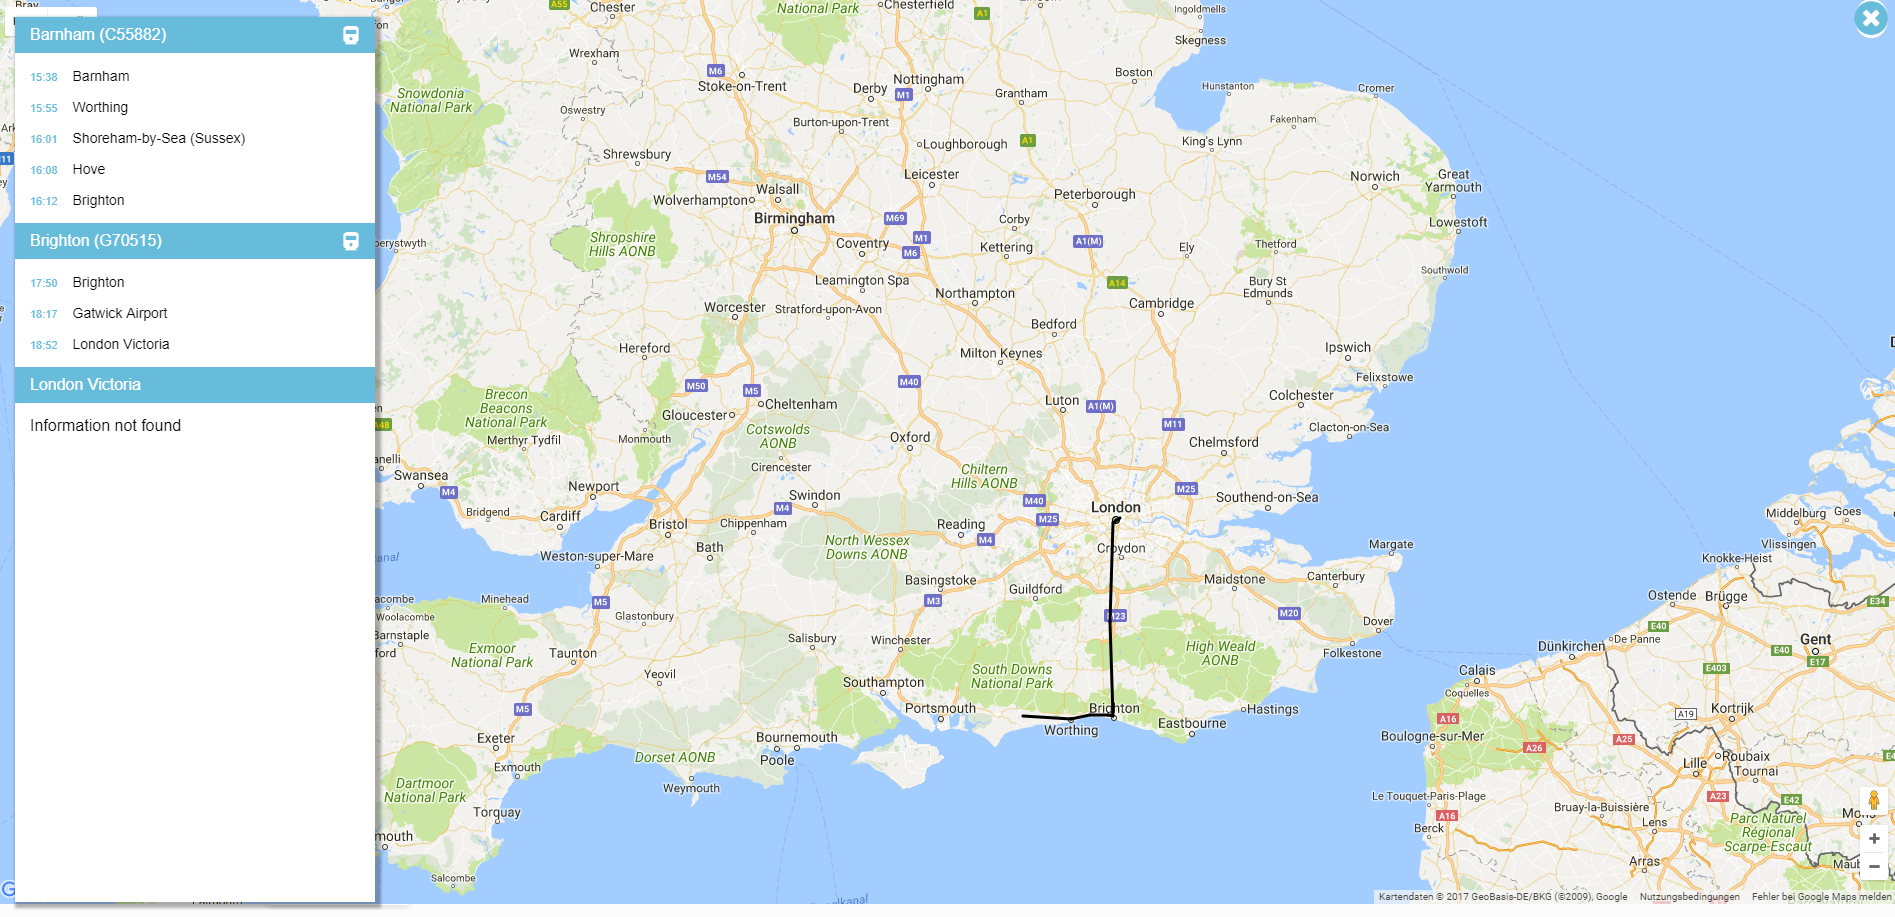
\includegraphics[width=16cm]{TrainticketsTO.png}
	\caption{Traintickets.To Webseite ~\cite{traintickets_site}}
	\label{fig:TrainticketsTO}
\end{figure}     


\subsection{Open Trip Planner}
\label{sec:OTP}

Der OpenTripPlanner kurz OTP ist eine auf der Maven-Repository ~\cite{maven_repository} aufbauende Multimodale trip planning Software welche anfangs für Städte ausgelegt war, nun aber auch in ersten landesweiten Netzwerken Anwendung findet. Er wurde von einem OpenSource-Kollektiv aus mehr als 100 Personen in acht Jahren entwickelt. ~\cite{otp_website}

Der OTP basiert auf dem A*-Algorithmus und verwendet GTFS-Daten und OpenStreetMap Daten in Form einer pbf-Datei. In einem preprocessing Schritt wird der Graph für den Algorithmus erstellt. Dieser kann in einer Datei gespeichert werden oder direkt im RAM des Servers gelagert werden. Selbiges wird für die OpenStreetMap-Daten gemacht. Während dem Betrieb kann der Graph angepasst werden, so dass das Programm auf verspätete Züge reagieren kann. ~\cite{otp_git}

OTP steht unter einer GNU Lesser General Public License. 

Vorteile des OTP sind, dass er in Echtzeit auf Fahrplanänderungen und Verspätungen reagieren kann, dass OTP schon seit mehreren Jahren in verschiedenen Städten implementiert und getestet ist und dass unsere Arbeit vom OpenSource-Kollektiv in den Hauptcode aufgenommen werden könnte. 

Nachteile des OTP sind, dass landesweite Implementationen erst in der Beta-Phase sind und somit noch nicht ausreichen getestet sind und dass das Programm unheimlich gross und verzweigt ist, so dass eine lange Einarbeitungszeit von Nöten ist.



\subsection{R5}
\label{sec:R5}

Rapid Realistic Routing on Real-world and Reimagined networks oder kurz R5 ist ein multimodales Trip-Planning-Tool. Er wurde von der Firma Conveyal ~\cite{conveyal} entwickelt und basiert auf dem OTP. 

R5 hat die Grundstruktur des OTP übernommen, jedoch verwendet R5 den RAPTOR-Algorithmus anstelle des A*-Algorithmus. Dadurch wurden einige Programmstrukturen verändert, da der RAPTOR-Algorithm nicht auf den Dijkstra-Algorithmus aufbaut und auch keinen Graphen verwendet. ~\cite{r5_git}

R5 steht unter der MIT License. 

Vorteile des R5 sind, dass er in Echtzeit auf Fahrplanänderung und Verspätungen reagieren kann und dass der RAPTOR-Algorithmus eine bessere Performance als die Dijkstra-basierten Algorithmen bietet. 

Nachteile des R5 sind, dass er unter einer MIT License steht und dass der R5 von einer Firma entwickelt wurde, welche unsere Arbeit nicht übernehmen werden.